\newpage
\section{Implementierung}

Wie in Abschnitt XX bereits erwähnt ist die Applikation dem Design-Pattern Model-View-Controller nachempfunden. Im Folgenden wird nun die konkrete Implementierung beschrieben und die Architektur mittels Codebeispielen konkretisiert.
\\
Der allgemeine Ablauf der Anwendung sieht lediglich einen Aufruf der HTML-Seite index.html vor. In diese wird mittels Javascript der jeweilige Inhalt (eine View) geladen und mit Daten und Funktionen (Controller) und versorgt.
\\
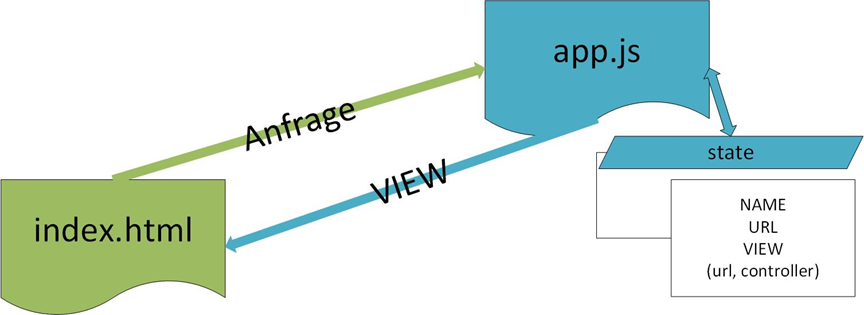
\includegraphics[width=1\textwidth]{ref/images/index.png} \\ 
App.js ist eine Javascript-Datei, die die Zuordnung der Views zu ihrem jeweiligen Controller durchführt. An dieser Stelle ist pro View ein Status (state) hinterlegt, der die Informationen hält (Name des Status, URL (innerhalb der App), View-Bezeichnung (URL der View, Controllername)). Die Informationen über die aktuell gewählte View gibt app.js an index.html zurück, welche sie nach außen dem Nutzer darstellt.
\\
App.js wird bei jedem Start der Applikation zuerst geladen. Dabei findet auch immer eine Prüfung der aktuellen Internetverbindung statt.
\\
Internet wird für die Darstellung des Kartenmaterials benötigt. Die Konsequenz einer fehlenden Internetverbindung ist demnach ein Abbruch der Applikation.
\\
Standardmäßig wird bei korrektem Startverhalten die play-View geladen. Das ist eine ebenfalls in App.js definierte Defaulteinstellung.
\\
Alle folgenden Statusbeschreibungen trennen View, Controller und Modell schematisch voneinander, wobei der Begriff Modell durch den Cordova-spezifischen Begriff Service ersetzt wird.
\\
Die App besitzt einen getabbten Aufbau, das heißt es existiert eine Kopfzeile, die dem Nutzer 4 verschiedene Tabs anbietet: Spielen, Highscores, Account und Credits. Jeder der Tabs wird im Folgenden näher beschrieben werden.
\subsection{Spielen}
Der Spielen-Tab bietet dem Nutzer die Möglichkeit sich für ein Spiel anzumelden. Er gibt dafür einen Namen und einen Spielradius an. Unter dieser Kombination wird er später seinen Highscore dieses Spiels finden können. Die View, die dahinter steht ist die Play-View, welche prinzipiell als Startseite der Applikation angezeigt wird. 
\subsubsection{Play}
Die Play-View hat ein Textfeld, dass den Spielernamen übernehmen kann und eine Selectbox, die den Radius auf zwei bis fünf Kilometern beschränkt. Bei fehlender Eingabe wird auf drei Kilometer als Defaultwert gesetzt. Außerdem bietet die View einen Button, der das Spiel startet. 
\\
Schon während der Eingabe der benötigten Informaitonen (Name und Radius) wird ein Objekt 'player' generiert, des diese Daten enthält, und mit Druck auf den Button an die Funktion savePlayer übergeben wird. Die Funktion 'savePlayer(p)' wurde der View durch den Controller 'PlayCtrl' (zugewiesen über app.js) bereitgestellt.
\\
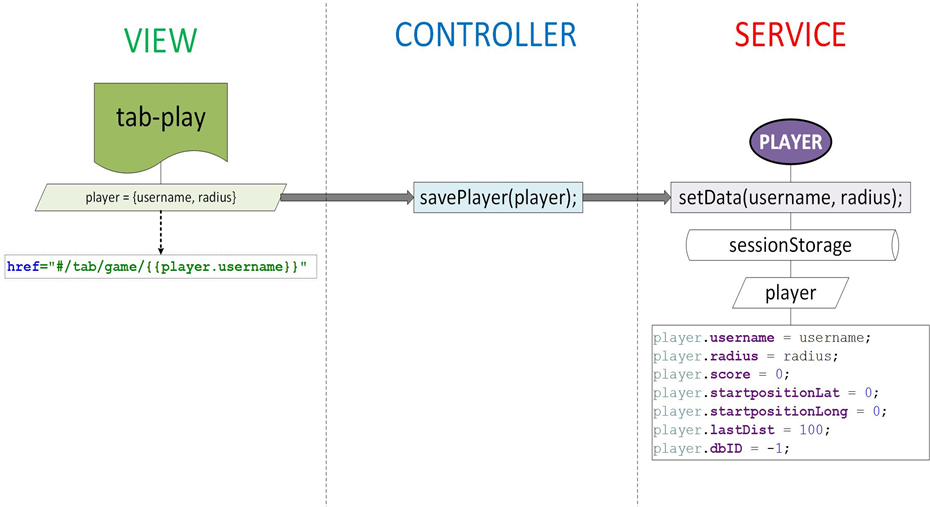
\includegraphics[width=1\textwidth]{ref/images/play.png} \\ 
\\
Der Controller leitet bei Aufruf dieser Funktion die Objektdaten Name und Radius an den dazugehörigen Service 'Player', der zuerst auf gültige Befüllung des Spielernamen prüft und bei Befüllung diesen speichert. Der genutzte Speicher ist der sessionStorage des Geräts, der für die Dauer der Session die Daten des Spielers als Objekt mit den folgenden Eigenschaften speichert: 

\begin{enumerate}
\item Spielername und Radius (beides über Nutzer eingegeben und über Controller an Service zur Speicherung übergeben)
\item Score
\item StartpositionLat (Breitengrad der Startposition)
\item startpositionLong (Längengrad der Startposition)
\item lastDist (letzte Distanz zum Ziel für Verlaufsvergleich)
\item dbID (ID des Spielers im Spielerarray des Sessionstorage)
\item lastUpdate (Zeitpunkt der letzten Änderung)
\end{enumerate}

Wenn der Spielername nicht angegeben wurde erhält der Nutzer eine Aufforderung und das Spielerobjekt wird nicht weitergeleitet und gespeichert. Bei erfolgreichem Speichern hingegen erfolgt eine Weiterleitung in den Zustand 'tab-game'.
\subsubsection{Game}
Die Game-View liegt ebenfalls im Tab 'Spielen' und ist für die aktuelle Standortbestimmung - also die Bestimmung des Startpunkts des Nutzers zuständig.


\subsubsection{Umsetzung iBeacons}
Ziel der Umsetzung in dieser Arbeit ist, dass die definierten Zielpunkte der App mit jeweils einem iBeacon ausgestattet werden.Damit diese die Genauigkeit der Entfernung verbessern.
Hierfür muss die App Signale des iBeacons empfangen. Deshalb läuft während der gesamten Ortungsphase im Hintergrund ein iBeacon Scanner. Sobald dieser Scanner den gewünschten iBeacon entdeckt hat wird die Distanz zum Ziel durch den iBeacon bestimmt und nicht per GPS, dadurch wird eine höhere Genauigkeit im Zielgebiet erreicht.

Um dies zu implementieren, muss das Zielpunkt Objekt angepasst werden. Standortobjekte benötigen neben Namen und Positionen noch eine iBeacon ID sowie Major und Minor Werte.

Mit den neuen Werten sind alle Vorraussetzungen geschaffen um einen iBeacon Scanner zu implementieren. Hierfür wird das Plug-In "Cordova / Phonegap iBeacon plugin" von Peter Metz verwendet. Es ist open Source und kann von Git Hub heruntergeladen werden.

Das Plug-In enthält Schnittstellen und Funktionen zum finden von iBeacons. Hierbei werden zwei unterschiedliche Funktionalitäten geboten.


1. Monitoring von iBeacons
Beim Monitoring wird ständig überprüft ob das Smartphone welches das Plug-In nutzt in einen Bereich eintritt, indem ein iBeacon Signale sendet. Ebenfalls wird überprüft ob das Smartphone den Bereich verlässt. Diese Funktion wird in dieser Arbeit genutzt um dem User anzuzeigen, dass bei Eintritt in eine iBeacon Zone nicht mehr GPS genutzt wird, sondern die Abstandsbestimmung mit Hilfe des iBeacons erfolgt.

2. Ranging von iBeacons
Während Monitoring nur den Aus- bzw. Einritt in eine Zone überprüft, ermittelt das iBeacon Ranging alle in der nähe befindlichen iBeacons und gibt eine ungefähre Distanz zu diesen an. Diese Funktionalität wird genutzt um die Distanz zum Zielort in der App darzustellen.\cite{MonitorRange}


Im folgenden wird die Umsetzung anhand von Quellcode Beispielen erläutert:

Installation
Damit das Plug-In genutzt werden kann, muss es erst über die Console des Betreibssystem installiert werden.

Hierfür navigiert man in der Console zum Hauptordner der App. Dort führt man den Befehl:

\begin{lstlisting}
cordova plugin add https://github.com/petermetz/cordova-plugin-ibeacon.git
\end{lstlisting} 


aus. Draufhin erfolgt die Automatische Installation im Ordner "plugin" der App und es kann auf die Schnittstellen zugegriffen werden.

Der allgemeine Ablauf besteht aus mehreren Schritten:
\begin{enumerate}
\item Schritt Anlegen eines Arrays mit iBeacon Informationen
\item Schritt Hauptfunktion mit for-Schleife aufrufen
\item Schritt Warten auf einen iBeacon in Reichweite
\item Schritt Gefundenes iBeacon-Objekt in Variable schreiben
\item Schritt Daten aus Objekt auslesen und anzeigen
\end{enumerate}



\underline{TODO: An dieser Stelle wird mit Code-Listings die Umsetzung dieser Schritte }\\
\underline{detailliert erläutert werden.}
